\documentclass[conference]{IEEEtran}
\usepackage{amsmath,amssymb}
\usepackage{graphicx}
\usepackage{subcaption}
\usepackage{booktabs}
\usepackage{cite}
\usepackage{xcolor}
\usepackage{stfloats}

\newcommand{\mat}[1]{\begin{bmatrix}#1\end{bmatrix}}
\setlength{\textfloatsep}{9pt plus 2pt minus 2pt}
\setlength{\floatsep}{8pt plus 2pt minus 1pt}
\setlength{\intextsep}{9pt plus 2pt minus 1pt}
\setlength{\abovecaptionskip}{4pt}
\setlength{\belowcaptionskip}{1pt}

\begin{document}

\title{Modelling, State Estimation, and Discrete LQR Control of a Self-Balancing Robot}

\author{
\IEEEauthorblockN{Fabian Dalenius, Kristoffer Liljendahl, Abdalrahman Nasser}
\IEEEauthorblockA{Department of Computer Science, Electrical and Space Engineering\\ Lule\aa\ University of Technology, R7003E}
}

\maketitle

\begin{abstract}
A MinSeg self-balancing robot is a wheel-mounted inverted pendulum that must be actively stabilised through wheel torque. This paper presents its non-linear and linearised modelling, and compares four control strategies: PID, pole-placement state feedback, continuous-time linear-quadratic regulation (LQR), and a discretised LQR with full-order and reduced-order Luenberger observers. The linearised model satisfies $\mathrm{rank}(\mathcal{C})=4$ (fully controllable) but only $\mathrm{rank}(\mathcal{O})=3$ when observed from the body angle alone, since the wheel position does not affect the angle dynamics; measuring both wheel position and body angle restores full observability. On the physical robot, PID kept the robot balanced for approximately 20~s of a 30~s test before falling, while the discretised LQR controller with a Luenberger-type observer remained balanced for the full 30~s recorded run, with motor voltage well inside the $\pm9$~V actuator limit. A sampling-frequency study found the robot could balance down to about 4.5~Hz on hardware, well below the 47.6~Hz an observer-inclusive simulation predicted was required; $f_s=200$~Hz was selected as the validated operating point. A discrete reference compensator tracked ramp references up to $r_{\max}=0.08$~m/s, but lost tracking under a demanding sinusoidal reference once the motor voltage approached saturation. LQR with observer-based estimation gave the most reliable physical performance of the strategies tested.
\end{abstract}

\begin{IEEEkeywords}
inverted pendulum, self-balancing robot, LQR, pole placement, Luenberger observer, discretization, reference tracking
\end{IEEEkeywords}

\section{Introduction}
A self-balancing robot is a wheel-mounted inverted pendulum: an open-loop unstable plant that must be actively stabilised through wheel torque. It is a compact but representative test bed for practical control engineering -- an unstable linear model that is only locally valid, sensors that do not cover the full state, an actuator with a hard voltage limit, and a digital controller running at a finite sampling rate.

The objective of this work is to design, implement, and experimentally evaluate a complete control chain for a MinSeg robot: derivation and linearisation of the equations of motion; a PID controller; a controllability/observability analysis; pole-placement and LQR state-feedback controllers; full-order and reduced-order Luenberger observers; discretisation; a sampling-frequency study; and a reference-tracking compensator for the wheel position. The toolkit is deliberately classical -- PID, pole placement, LQR \cite{anderson}, and Luenberger observation \cite{luenberger}, discretised by zero-order hold \cite{franklin} -- so as to characterise how far a strictly linear design can be pushed before sampling limits, noise, and actuator saturation cause it to fail.

The central question is: \emph{how do PID, pole-placement, and LQR control, combined with different observer structures, compare on a real balancing robot, and how do sampling frequency, saturation, and model uncertainty affect performance?} Section~\ref{sec:model} presents the model. Section~\ref{sec:design} presents the controllers and observers. Section~\ref{sec:discrete} covers discretisation and the sampling-frequency study. Section~\ref{sec:results} reports the physical experiments and reference tracking. Sections~\ref{sec:discussion}--\ref{sec:conclusion} discuss and conclude.

\section{System Model}\label{sec:model}
\begin{figure}[t]
\centering
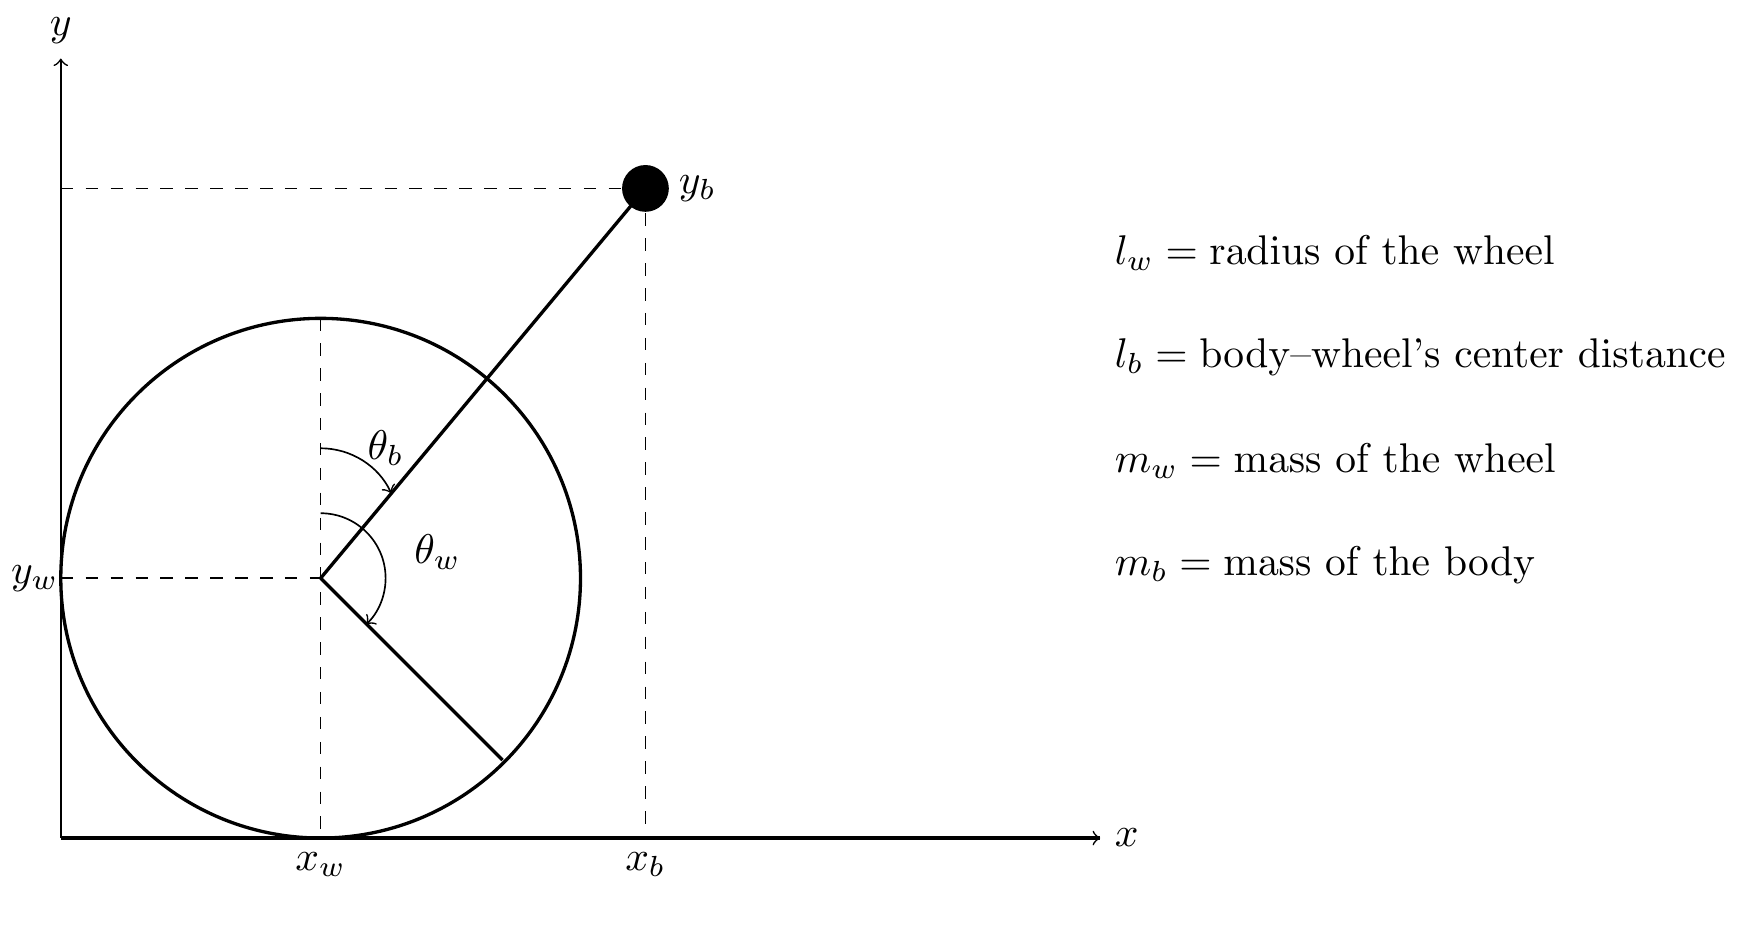
\includegraphics[width=0.8\linewidth]{../fig/schematic.png}
\caption{Planar model of the robot: body angle $\theta_b$, wheel angle $\theta_w$, wheel radius $l_w$, body--wheel distance $l_b$.}
\label{fig:schematic}
\end{figure}

The robot (Fig.~\ref{fig:schematic}) is modelled as a point mass $m_b$ at distance $l_b$ from the wheel centre, plus a wheel of mass $m_w$ and radius $l_w$ driven by a DC motor of resistance $R_m$, torque constant $K_t$ and back-emf constant $K_e$. With motor and friction torque
\begin{align}
T_m &= \tfrac{K_t}{R_m}v_m - \tfrac{K_eK_t}{R_m}\big(\tfrac{\dot x_w}{l_w}-\dot\theta_b\big), &
T_f &= b_f\big(\tfrac{\dot x_w}{l_w}-\dot\theta_b\big),
\end{align}
Newton--Euler analysis of the wheel and body gives, with $J_b\equiv I_b+m_bl_b^2$ and $J_w\equiv I_w/l_w+l_wm_b+l_wm_w$,
\begin{align}
J_b\ddot\theta_b + m_bl_b\ddot x_w\cos\theta_b &= m_bl_bg\sin\theta_b - T_m + T_f,\\
J_w\ddot x_w + m_bl_bl_w\ddot\theta_b\cos\theta_b &= m_bl_bl_w\dot\theta_b^2\sin\theta_b + T_m - T_f.
\end{align}
The $\sin\theta_b$ factor on the centripetal term in the wheel equation follows from the non-linear kinematics of the body's centre of mass. Under the small-angle approximation below, this term becomes proportional to $\dot\theta_b^2\theta_b$ and is neglected as a higher-order product.

The system is linearised about the upright equilibrium $\theta_b=0,\ \dot\theta_b=0,\ \dot x_w=0$, using $\sin\theta_b\approx\theta_b$, $\cos\theta_b\approx1$, and neglecting products of small variables such as $\dot\theta_b^2\theta_b$. With $x=[x_w,\dot x_w,\theta_b,\dot\theta_b]^{\mathsf T}$, the linearised equations can be written compactly as an equation for the two accelerations,
\begin{equation}
\gamma\mat{\ddot x_w\\\ddot\theta_b} = \alpha x + \beta v_m,
\end{equation}
with $\gamma\in\mathbb{R}^{2\times2}$ the inertia matrix, $\alpha\in\mathbb{R}^{2\times4}$ the state coefficients, and $\beta\in\mathbb{R}^{2\times1}$ the input coefficients. Solving for $[\ddot x_w,\ddot\theta_b]^{\mathsf T}$ and inserting into rows 2, 4 of the state-space model (rows 1, 3 being the kinematic identities $\dot x_w=x_2$, $\dot\theta_b=x_4$) gives
\begin{equation}
\dot x = Ax+Bv_m,\qquad y = Cx.
\end{equation}
Using the parameters of Table~\ref{tab:params}, this evaluates to
\begin{equation}
A=\mat{0&1&0&0\\0&-435&-6.1&9.1\\0&0&0&1\\0&1903.4&62&-40},\quad
B=\mat{0\\20.576\\0\\-90.028},
\end{equation}
which match the model used throughout the group's laboratory work. Because the first column of $A$ is zero, $x_w$ does not influence $\dot x_w,\theta_b,\dot\theta_b$: it is driven by, but never feeds back into, the pendulum dynamics. Retaining only $\theta_b$ as output ($C_\theta=[0\;0\;1\;0]$) and eliminating the unforced $x_w$ state gives the transfer function
\begin{equation}
G(s)=\frac{\theta_b(s)}{v_m(s)}\approx\frac{-90.03\,s}{(s-5.72)(s+5.66)(s+475.07)},
\end{equation}
obtained by direct evaluation of $C_\theta(sI-A)^{-1}B$: it has an unstable real pole at $+5.72\ \text{rad/s}$, a stable pole at $-5.66\ \text{rad/s}$, a fast motor pole at $-475.07\ \text{rad/s}$, and a zero within $10^{-3}$ of the origin, inherited from the $x_w$ integrator.

\subsection{Disturbance Input}
To study robustness against an external push (e.g.\ a poke), a second input $F_d$ acting on the body was added via an extended input matrix
\begin{equation}
u=\mat{v_m\\F_d},\qquad
B_{\text{ext}}=\mat{0&0\\20.576&2.105\\0&0\\-90.028&2.026}.
\end{equation}
Since its two columns are not parallel, $F_d$ cannot be represented as an equivalent change in motor voltage: it excites a different direction in the state space than $v_m$, although closed-loop feedback may still reject the resulting state deviation.

\begin{table}[t]
\centering
\caption{Physical parameters used throughout.}
\label{tab:params}
\footnotesize
\setlength{\tabcolsep}{2pt}
\begin{tabular}{@{}llll@{}}
\toprule
$g=9.8\,\mathrm{m/s^2}$ & $m_b=0.381\,\mathrm{kg}$ & $l_b=0.112\,\mathrm{m}$ & $I_b=0.00616\,\mathrm{kg\,m^2}$\\
$m_w=0.036\,\mathrm{kg}$ & $l_w=0.021\,\mathrm{m}$ & $I_w=7.46\!\times\!10^{-6}$ & $R_m=4.4\,\Omega$\\
$K_e=0.444$ & $K_t=0.470$ & $b_f=0$ & $L_m=b_m=0$\\
\bottomrule
\end{tabular}
\end{table}

\section{Controller and Observer Design}\label{sec:design}
\subsection{PID Controller}
Pole placement on $G(s)$ -- moving the two stable poles to $-475,-5.66$ (unchanged) and the unstable pole to $-5$ -- gives the analytic PID gains $(K_d,K_p,K_i)=(-0.1191,-57.25,-320.23)$. On the physical robot these were retuned to $(K_d,K_p,K_i)=(-0.1191,-61.25,-340.23)$. With this controller the robot remained balanced for approximately 20~s of the 30~s test, with a modest motor swing ($|v_m|\lesssim5$~V), before the angle drifted past recovery and the robot settled on its side (Fig.~\ref{fig:pid}).

A proportional controller alone does not provide sufficient freedom to stabilise the stated angle-output model under the implemented feedback convention $v_m=-Kx$: for $G(s)=Ks/D(s)$ with $D(s)=s^3+475.0s^2-62.0s-15371.3$, a pure proportional loop gives closed-loop characteristic polynomial $D(s)-K_pKs$, whose constant term equals $D(0)=-15371.3$ regardless of $K_p$, so it cannot satisfy the necessary sign conditions for stability. A full PID controller was therefore designed to allow independent adjustment of the relevant characteristic-polynomial coefficients. Because the feedback signal contains only $\theta_b$, the absolute wheel-position state $x_w$ remains marginally stable and is not actively returned to the origin; this is consistent with the wheel visibly wandering in Fig.~\ref{fig:pid} and is a likely contributor to the eventual fall, once accumulated drift and the non-linear dynamics outside the small-angle region interact.

\begin{figure}[t]
\centering
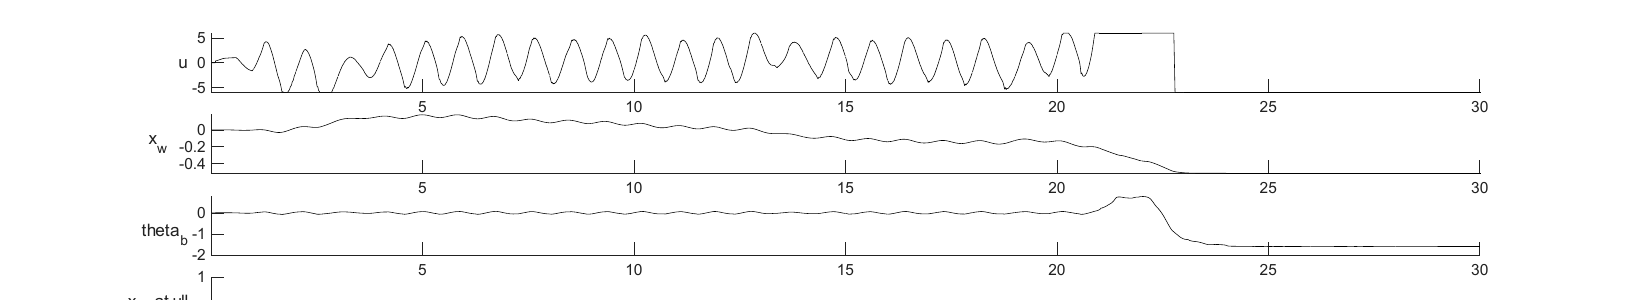
\includegraphics[width=0.98\linewidth]{../fig/pid_uxwtheta.png}
\caption{Physical PID test: motor voltage $v_m$, wheel position $x_w$, and body angle $\theta_b$ over 30~s. The robot balances for $\approx\!20$~s, then falls near $t\approx22$~s.}
\label{fig:pid}
\end{figure}

\subsection{Controllability and Observability}
With $C_\theta=[0\;0\;1\;0]$, the controllability matrix $\mathcal{C}=[B\;AB\;A^2B\;A^3B]$ satisfies $\mathrm{rank}(\mathcal{C})=4$ (fully controllable), while the observability matrix $\mathcal{O}=[C_\theta;C_\theta A;C_\theta A^2;C_\theta A^3]^{\mathsf T}$ satisfies $\mathrm{rank}(\mathcal{O})=3$. The unobservable state is $x_w$: since column~1 of $A$ is zero, no combination of $\theta_b$ measurements can reveal the wheel position, which also explains the pole-zero cancellation at $s=0$ in $G(s)$. Measuring $x_w$ in addition to $\theta_b$ (wheel encoder and gyro/accelerometer) gives the two-output matrix
\begin{equation}
C_m = \mat{1&0&0&0\\0&0&1&0},
\end{equation}
which restores full observability and is used for both observers below. A separate matrix $C_r=[-1\;0\;0\;0]$ is used later for the reference compensator, which regulates $x_w$.

\subsection{Pole-Placement State Feedback}
Assuming full state feedback $v_m=-Kx$, a dominant second-order pair was placed at $-5.66\pm j5.78$ ($\zeta=0.7$), backed by two fast poles at $-470,-480$. Using \texttt{place(A,B,p)} on the full-precision model of Section~\ref{sec:model} gives
\begin{equation}
K_{\text{pp}} = \mat{-20307.89 & -3618.66 & -7267.51 & -832.45},
\end{equation}
for which $\mathrm{eig}(A-BK_{\text{pp}})=\{-480,-470,-5.66\pm j5.78\}$. The gain was calculated from the full-precision model; using the unrounded gain gives the intended closed-loop poles, while the matrices shown in Section~\ref{sec:model} are rounded for presentation. This gain drives $\theta_b,x_w$ to zero within about $1.5$~s (Fig.~\ref{fig:compare}, top row) at the cost of large transient effort.

\subsection{Linear-Quadratic Regulator}
An LQR $v_m=-Kx$ was designed via $K=\mathrm{lqr}(A,B,Q,R)$ with diagonal state weights $Q=\mathrm{diag}(30,1,150,7)$, $R=1$ (heaviest weight on $\theta_b$, since falling is the primary failure mode, with a smaller non-zero weight on $x_w$ to bound drift), giving
\begin{equation}
K_{\text{lqr}} = \mat{-5.477 & -44.333 & -66.861 & -10.885}.
\end{equation}
The closed-loop eigenvalues of $A-BK_{\text{lqr}}$ are $\{-531.8,-0.259,-5.34\pm j0.68\}$: the complex pair is nearly critically damped ($\zeta\approx0.99$), but the dominant mode is the \emph{real} pole at $-0.259$~rad/s ($\tau\approx3.9$~s), not a complex pair -- this explains the slow residual settling of $x_w$ in simulation. Compared with pole placement, LQR reduces the peak angle excursion ($-0.04$ vs.\ $-0.16$~rad) and peak voltage ($0.23$ vs.\ $0.4$~V) at the cost of that slow $x_w$ recovery (Fig.~\ref{fig:compare}, bottom row). LQR was selected for subsequent work mainly because weight tuning does not require guessing pole locations by hand.

\begin{figure}[t]
\centering
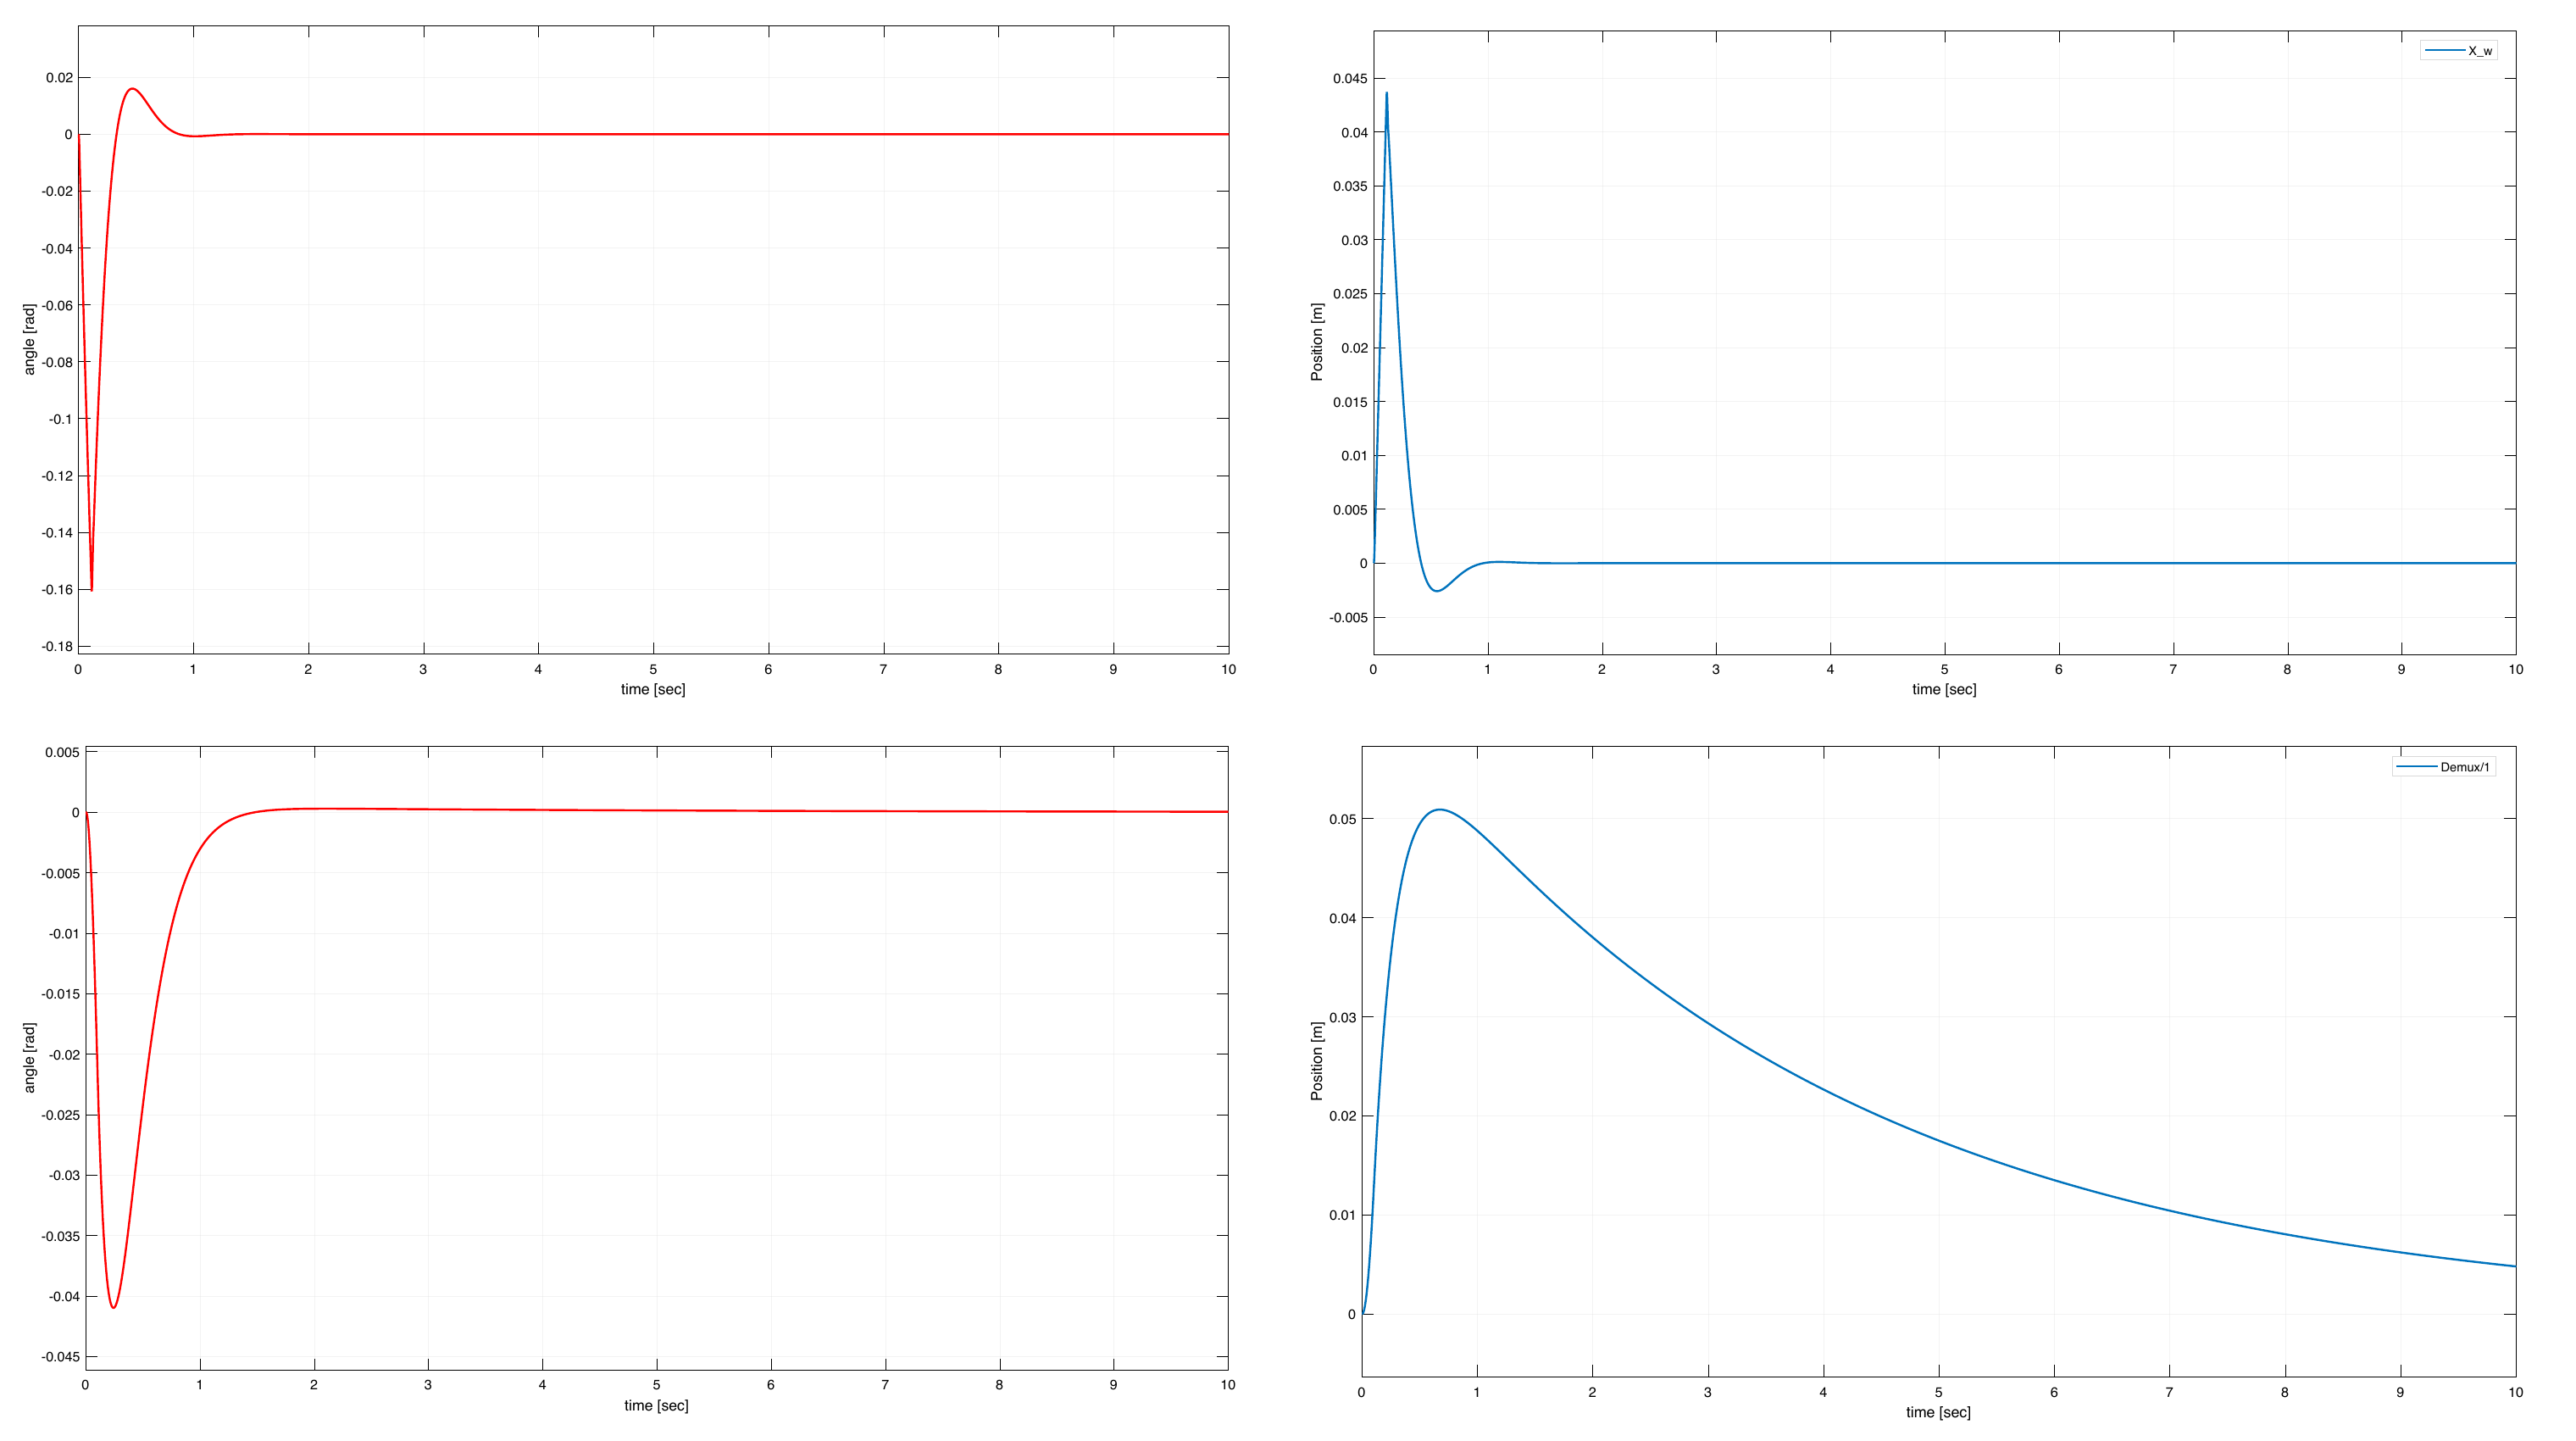
\includegraphics[width=0.92\linewidth]{../fig/compare_controllers.png}
\caption{Simulated step response to an initial angle offset. Top row: pole placement ($\theta_b$ left, $x_w$ right); bottom row: LQR ($\theta_b$ left, $x_w$ right). LQR trades a slower $x_w$ recovery for a smaller angle and voltage transient.}
\label{fig:compare}
\end{figure}

\subsection{State Observers}
The wheel position $x_w$ and body angle $\theta_b$ are measured directly (via $C_m$), while the wheel translational velocity $\dot x_w$ and the body angular velocity $\dot\theta_b$ are estimated. A full-order Luenberger observer
\begin{equation}
\dot{\hat x}=A\hat x+Bv_m+L(y-C_m\hat x)
\end{equation}
estimates the complete state vector and was designed by pole placement at $\{-513.8,-475,-4.71\pm j0.048\}$, using the duality $\mathcal{O}_{(A,C_m)}=\mathcal{C}_{(A^{\mathsf T},C_m^{\mathsf T})}^{\mathsf T}$ so that $L=\mathrm{place}(A^{\mathsf T},C_m^{\mathsf T},p)^{\mathsf T}$:
\begin{equation}
L = \mat{5.22&14.64\\-8.85&45.26\\17.07&517.99\\126.72&2477.39},
\end{equation}
computed from $L=\mathrm{place}(A^{\mathsf T},C_m^{\mathsf T},p)^{\mathsf T}$ on the full-precision model. The unrounded observer gain places the estimation-error poles $\mathrm{eig}(A-LC_m)$ at the selected locations $\{-513.8,-475,-4.71\pm j0.048\}$ (all negative real part). These poles were selected substantially faster than the controller's true dominant mode at $-0.259$ (Section~III-D) -- about $18\times$ faster for the slow observer pair, and far faster still for the $-475,-513.8$ pair -- while avoiding even more aggressive placement that could further amplify measurement noise.

A reduced-order observer was also built, treating the measured $x_w$ as exact and estimating $(\dot x_w,\theta_b,\dot\theta_b)$ with poles $\{-475,-4.71\pm j0.048\}$, giving gain matrices $M_1,\dots,M_7$ (omitted for space); $\theta_b$ is re-estimated here, even though it is directly measured, because the angle measurement is comparatively more affected by sensor noise than the encoder-based $x_w$ reading. This reduces the observer order from four estimated states to three, not from four to two. In simulation the full-order observer had a lower reported $\theta_b$ error than the reduced-order observer (max.\ $\approx$0.0017~rad); both tracked $x_w$ with negligible error (Fig.~\ref{fig:observer}). Which variant was used in the best physical run (Section~\ref{sec:results}) is not identified in the available laboratory record. With output noise $n_{\text{dist}}$ the error dynamics are $\dot e=(A-LC_m)e-Ln_{\text{dist}}$, $e=x-\hat x$: placing $L$ far to the left speeds convergence but also amplifies $n_{\text{dist}}$.

\begin{figure}[t]
\centering
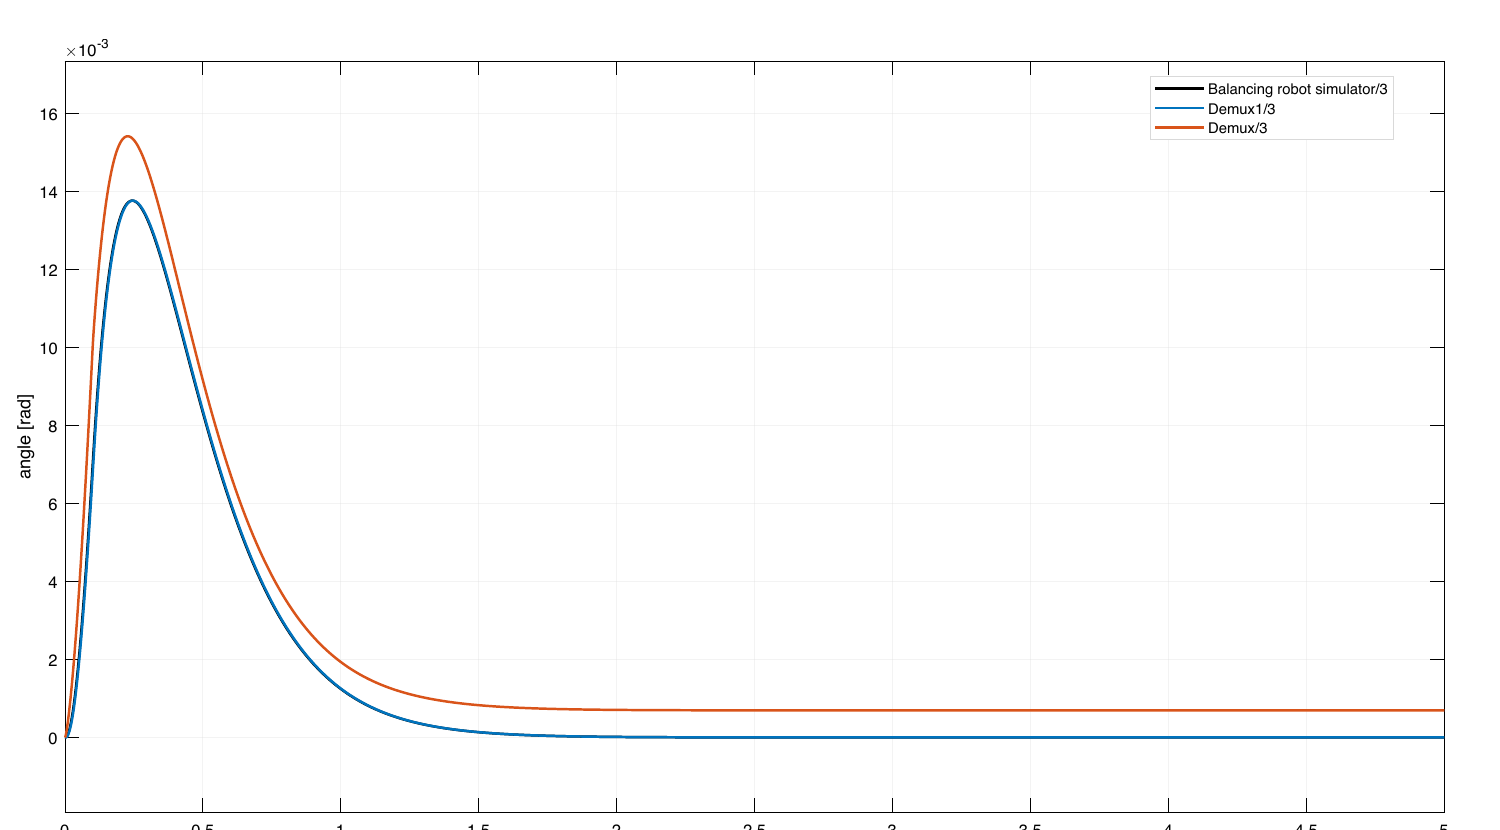
\includegraphics[width=0.9\linewidth]{../fig/observer_theta.png}
\caption{Simulated $\theta_b$: true state (black, overlapped) vs.\ full-order (blue) and reduced-order (orange) observer estimates.}
\label{fig:observer}
\end{figure}

\section{Discretization and Sampling Frequency}\label{sec:discrete}
The continuous plant was discretised using zero-order hold, $A_d=e^{AT_s}$, $B_d=\int_0^{T_s}e^{A\tau}d\tau\,B$, at $f_s=200$~Hz ($T_s=5$~ms), the rate ultimately used for the plant and state-feedback controller. The discrete feedback gain used for implementation at this rate,
\begin{equation}
K_d = \mat{-16.141 & -26.514 & -87.152 & -6.235},
\end{equation}
was taken from the Lab C implementation and verified to place all closed-loop eigenvalues of $A_d-B_dK_d$ strictly inside the unit circle, with largest magnitude $0.999$ -- indicating a very slowly decaying discrete mode rather than a strong stability margin. Discrete observer matrices $L_d$ and $M_{d,1..7}$ were developed separately, as part of the sampling-frequency investigation of this section: the version recorded in the laboratory report was computed for $T_s=0.021$~s ($f_s\approx47.6$~Hz), reusing the 200~Hz gain $K_d$ above rather than a rate-matched one. No separate observer design at $T_s=5$~ms is documented, so the exact discrete observer matrices used together with the 200~Hz controller in the physical run of Section~\ref{sec:results} cannot be confirmed from the written record.

\begin{table}[t]
\centering
\caption{Minimum stabilising sampling frequency under different scenarios (simulation vs.\ physical robot).}
\label{tab:freq}
\footnotesize
\setlength{\tabcolsep}{2pt}
\begin{tabular}{@{}lcc@{}}
\toprule
Scenario & $T_s$ [s] & $f_s$ [Hz]\\
\midrule
State feedback only, sim.\ (re-tuned $K_d$/rate) & 0.224 & 4.46\\
State feedback + observer, sim.\ (fixed $K_d$) & 0.021 & 47.6\\
State feedback + observer, physical robot & $\approx$0.22 & $\approx$4.5\\
Selected final operating point & 0.005 & 200\\
\bottomrule
\end{tabular}
\end{table}

Table~\ref{tab:freq} distinguishes five sampling-frequency values found at different stages, which must not be conflated. With exact state feedback and no observer, reducing $T_s$ from the 200~Hz baseline while re-optimising $K_d$ at each rate keeps the simulator stable down to $f_s\approx4.46$~Hz. Adding the observer -- while keeping the controller fixed at its 200~Hz design and only re-discretising the plant/observer at the test rate -- raises the simulated stability boundary to $f_s\approx47.6$~Hz. The physical robot, by contrast, remained balanced down to $f_s\approx4.5$~Hz -- close to the controller-only theoretical limit and well below the 47.6~Hz the observer-inclusive simulation predicted was required. Several factors could contribute to this gap: the controller and observer implementation used in the physical low-frequency test may not exactly match the fixed-$K_d$ simulation condition, sensor filtering and finite test duration may mask slow divergence, and floor friction and actuator deadband are not represented in the linear model. The available data do not isolate which of these dominates.

\begin{figure}[t]
\centering
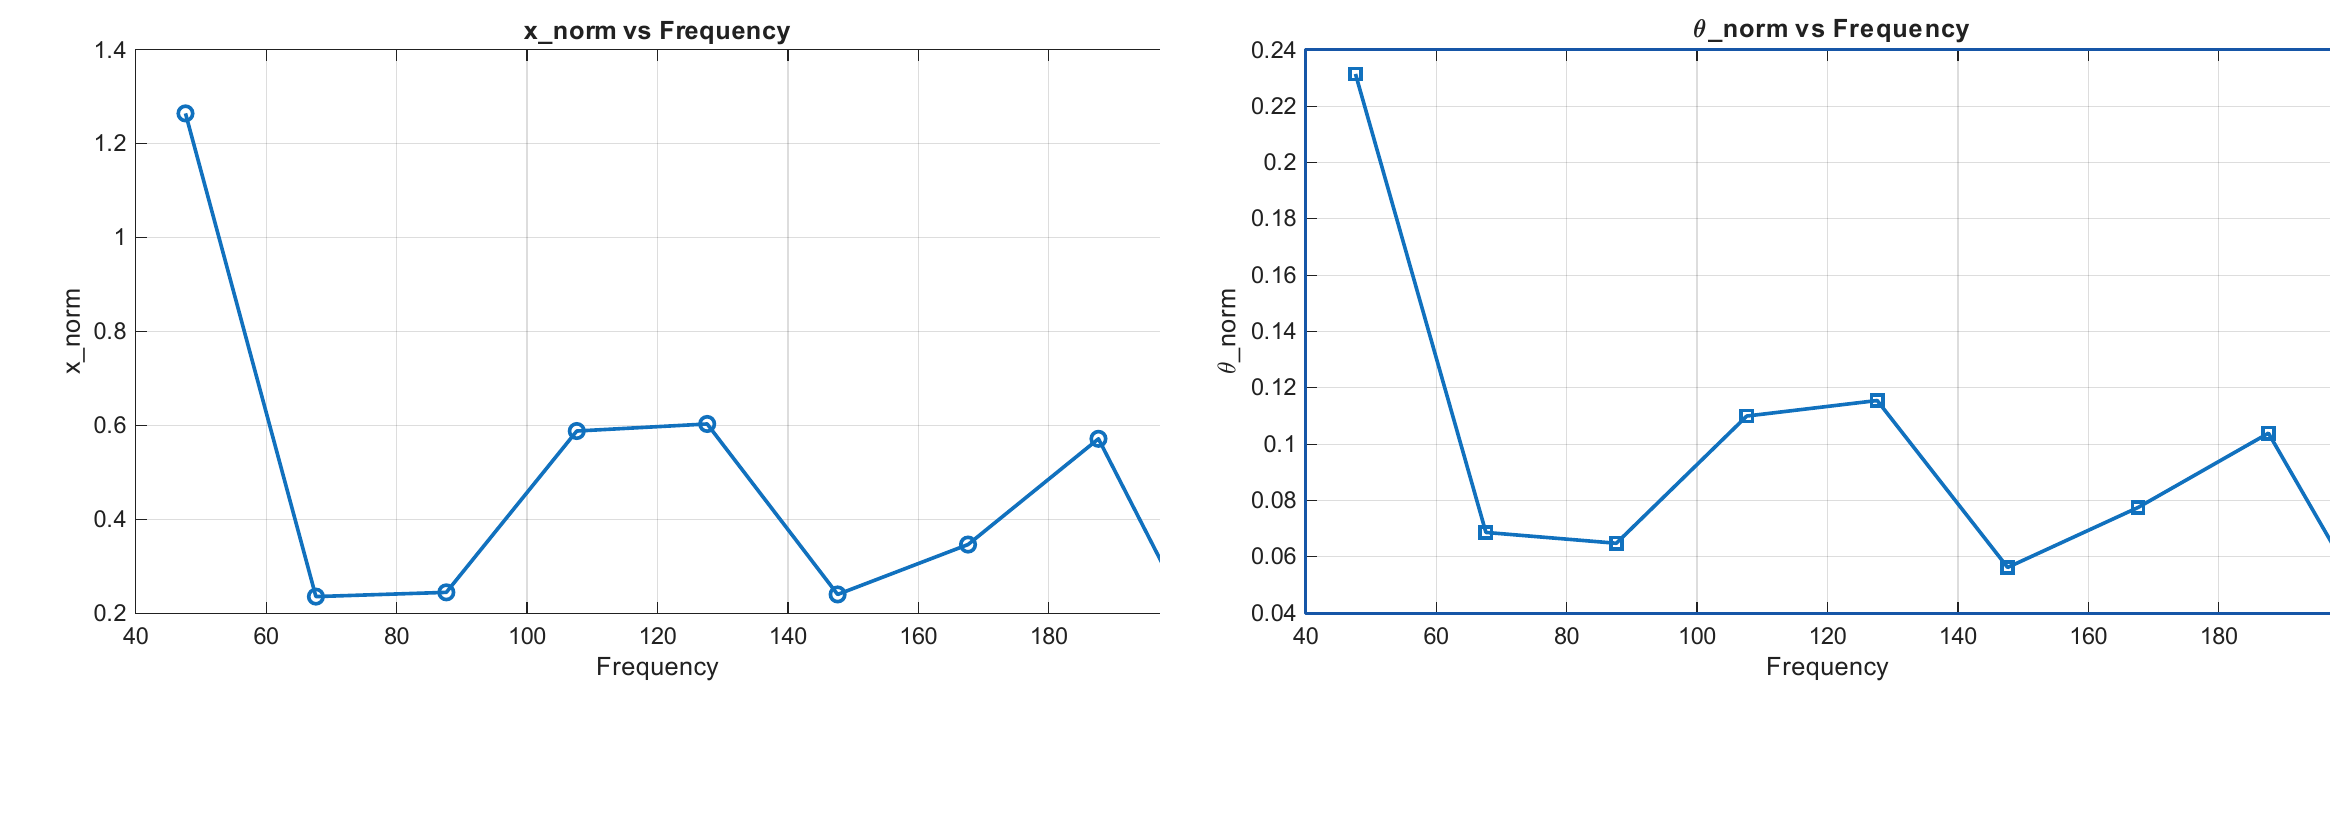
\includegraphics[width=0.98\linewidth]{../fig/l2_norms_combined.png}
\caption{$L_2$-norm of $x_w$ (left) and $\theta_b$ (right) over a 30~s balancing test, for nine sampling frequencies from 47.6--200~Hz on the physical robot.}
\label{fig:l2norm}
\end{figure}

A further sweep on the physical robot, raising $f_s$ from 47.6~Hz to 200~Hz in $\approx$20~Hz steps and computing the $L_2$-norm $\|\cdot\|_2=\sqrt{\sum_k x[k]^2}$ of $x_w$ and $\theta_b$ over each 30~s trial (Fig.~\ref{fig:l2norm}), shows a non-monotonic relationship: both norms are high near 47.6~Hz, drop near 70--90~Hz, rise again around 110--190~Hz, and are again low at 200~Hz -- comparably low to the 70--90~Hz band, not uniquely lowest. Each frequency was a single 30~s trial rather than an ensemble average, so run-to-run variability in initial angle, floor grip, and disturbance timing can shift individual points substantially. $f_s=200$~Hz was selected as the final operating frequency because it produced low measured norms for both $x_w$ and $\theta_b$ and was already the validated operating frequency for the plant and state-feedback controller. The sampling-frequency sweep did not establish a unique global optimum.

\section{Experimental Results}\label{sec:results}
\subsection{Balancing Performance}
With the discrete LQR controller, a Luenberger-type observer, and $f_s=200$~Hz, the robot remained balanced throughout the full 30~s recorded run, with motor voltage swinging by about 5~V peak-to-peak (roughly $\pm2.5$~V about zero) -- well inside the $\pm9$~V actuator limit -- and the wheel position drifting only within roughly $-0.12$ to $0$~m (Fig.~\ref{fig:best}). The available record does not identify whether the full-order or the reduced-order Luenberger observer was used for this run, nor the exact discrete observer matrices applied together with the 200~Hz controller (Section~\ref{sec:discrete}). The robot was also qualitatively reported to recover from manual disturbances and to balance on an inclined surface, although no recorded signals from these tests were available for quantitative evaluation.

\begin{figure}[t]
\centering
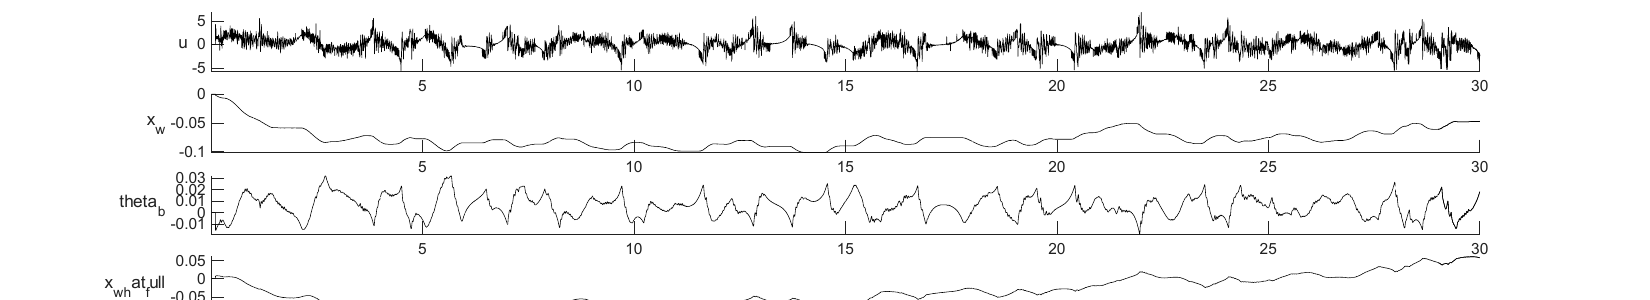
\includegraphics[width=0.98\linewidth]{../fig/best_uxwtheta.png}
\caption{Best physical balancing run: motor voltage $v_m$, wheel position $x_w$, body angle $\theta_b$ (30~s, $f_s=200$~Hz, LQR with Luenberger observer).}
\label{fig:best}
\end{figure}

\subsection{Reference Compensator}
To make $x_w$ track a position reference with zero discrete-time steady-state error, a steady-state target state $N_x$ and input $N_u$ are found from $x_{ss}=A_dx_{ss}+B_du_{ss}$, $r=C_rx_{ss}$. The wheel's positive-displacement convention is opposite to the plotted reference direction, so the tracked output is $y_r=-x_w$, i.e.\ $C_r=[-1\;0\;0\;0]$:
\begin{equation}
\mat{N_x\\N_u} = \mat{A_d-I & B_d\\ C_r & 0}^{-1}\mat{0\\1}.
\end{equation}
With the 200~Hz $A_d,B_d$ of Section~\ref{sec:discrete}, this gives $N_x=[-1,0,0,0]^{\mathsf T}$, $N_u=0$. The implemented control law is $v_m=-K_dx+Nr$, and evaluating it at steady state ($x=N_xr$) gives the scalar feed-forward gain $N=N_u+K_dN_x$. With $N_u=0$ and $N_x$ selecting the negated first entry of $K_d$, $N=-K_d(1,1)=16.141$, so $v_m=-K_dx+16.141\,r$; in steady state this yields $x_w=-r$, consistent with the encoder convention.

\subsection{Reference Tracking}
Three position references $r$ (metres) were tested in closed-loop runs on the physical robot; two representative experiments are shown in Figs.~\ref{fig:ref1} and~\ref{fig:ref3}. The first is a triangular ramp from 0 to 2~m and back over 120~s (Fig.~\ref{fig:ref1}); $x_w$ follows it closely throughout with $x_w\approx-r$, $\theta_b$ stays within about $\pm0.05$~rad, and $v_m$ stays within roughly $\pm8$~V, approaching but not clearly exceeding the $\pm9$~V rail. A second triangular reference to 2.5~m (not shown) produced comparable tracking. The third, more demanding reference is sinusoidal, amplitude 0.3~m, period $\approx$20~s (Fig.~\ref{fig:ref3}). Here $v_m$ reaches its plotted $\pm10$~V axis limits and stays there for extended stretches from about $t=40$~s onward -- the voltage command was at or beyond the $\pm9$~V actuator rating -- while $\theta_b$ moves far outside the small-angle region, reaching about $-1.4$~rad near $t\approx45$~s and about $-1.6$~rad near $t\approx60$~s before partially recovering; $x_w$ does not track the reference after this point and instead drifts to about $-9$~m by $t\approx120$~s. The group attributed the failure to the controller lagging the fast reference and then over-correcting once saturated, consistent with the observed timing.

\begin{figure*}[t]
\centering
\begin{subfigure}[t]{0.48\textwidth}
\centering
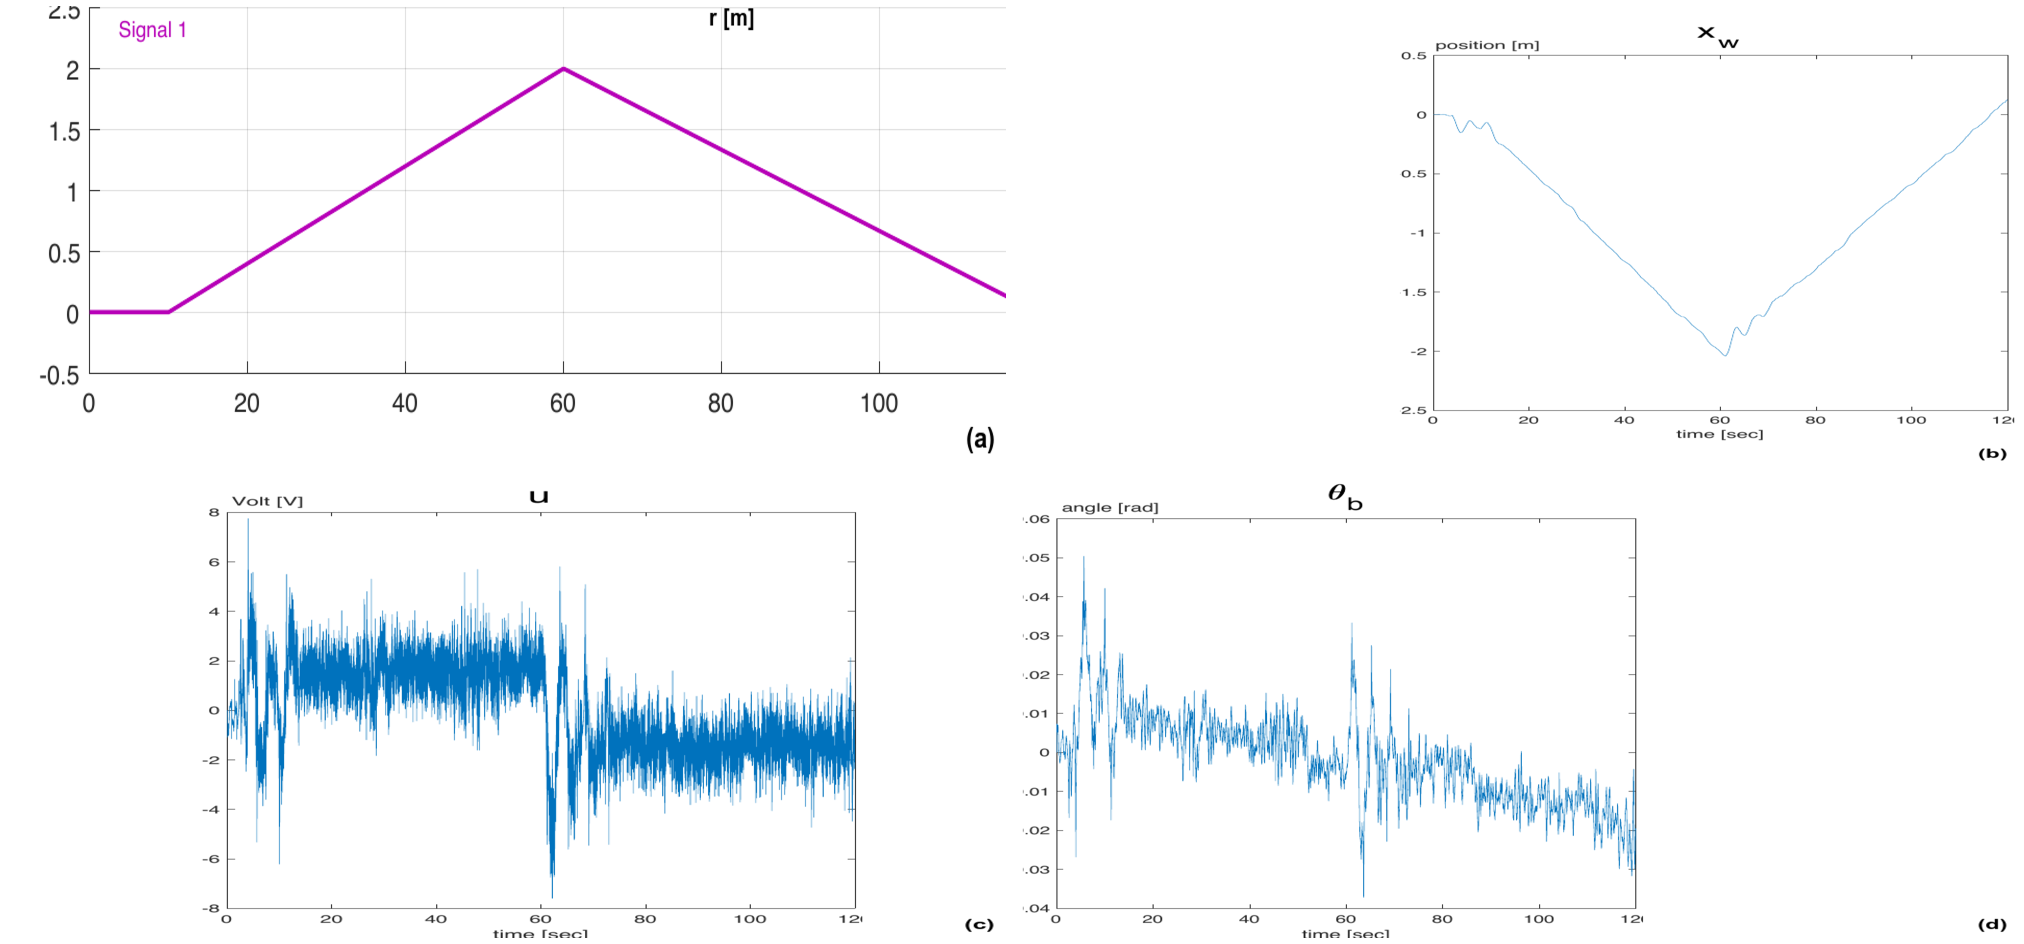
\includegraphics[width=\linewidth]{../fig/panel4_signal1.png}
\caption{Successful tracking: triangular $r$.}
\label{fig:ref1}
\end{subfigure}
\hfill
\begin{subfigure}[t]{0.48\textwidth}
\centering
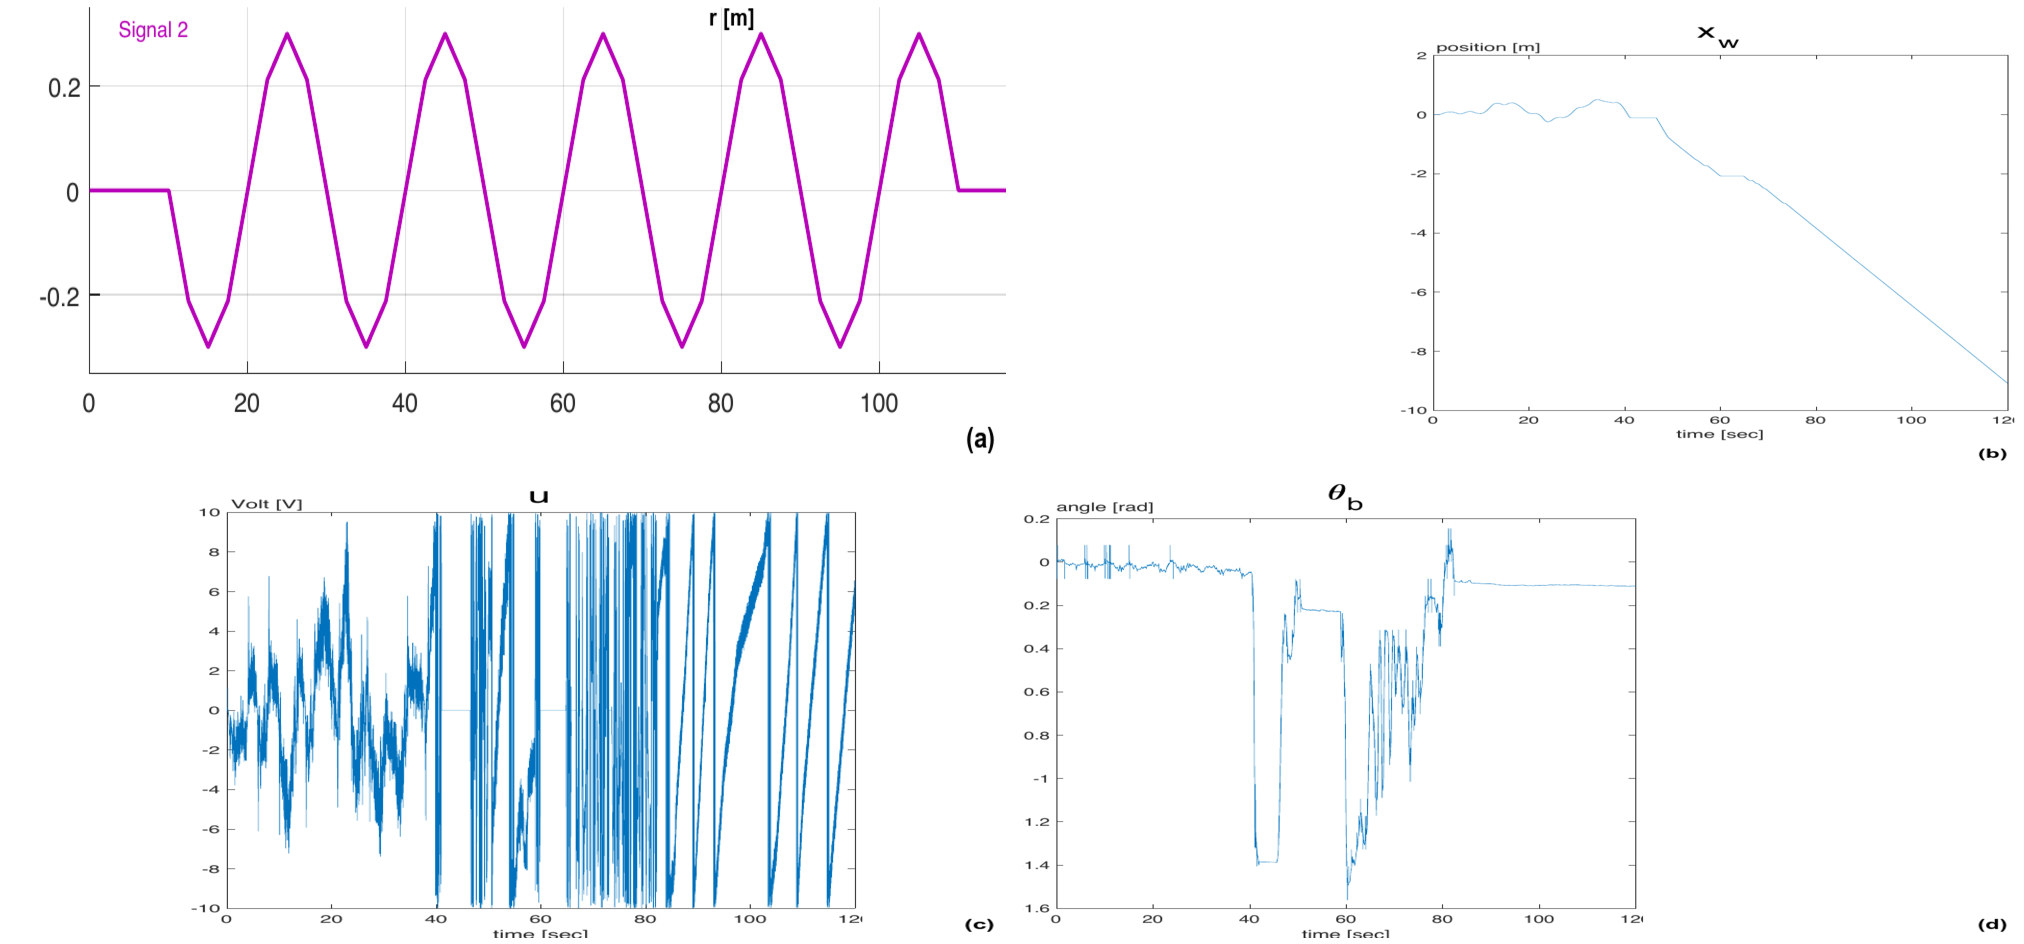
\includegraphics[width=\linewidth]{../fig/panel4_signal3.png}
\caption{Failed tracking: sinusoidal $r$.}
\label{fig:ref3}
\end{subfigure}
\caption{Reference tracking: (a) reference $r$, (b) wheel position $x_w$, (c) motor voltage $v_m$, (d) body angle $\theta_b$, over 120~s. Left: triangular reference, tracked closely. Right: sinusoidal reference -- $v_m$ reaches its $\pm10$~V axis limits (at or beyond the $\pm9$~V rating) and $\theta_b$ shows large excursions, after which $x_w$ stops tracking.}
\label{fig:reftrack}
\end{figure*}

In the separate final-demonstration test (Section~VI of the underlying lab instructions), $r$ is a ramp in $x_w$ whose \emph{slope} (m/s), not amplitude, is the tested parameter; the maximum ramp speed the robot could follow without falling was found by trial and error to be $r_{\max}=0.08$~m/s. Figure~\ref{fig:findemo} shows the measured $x_w$ against the commanded ramp for the standard test (slope 0.05~m/s, reaching $-0.5$~m) and the $r_{\max}$ test (slope 0.08~m/s, reaching $-0.8$~m); both were tracked with only small (2--5~cm) residual oscillation and without the robot falling.

\begin{figure}[t]
\centering
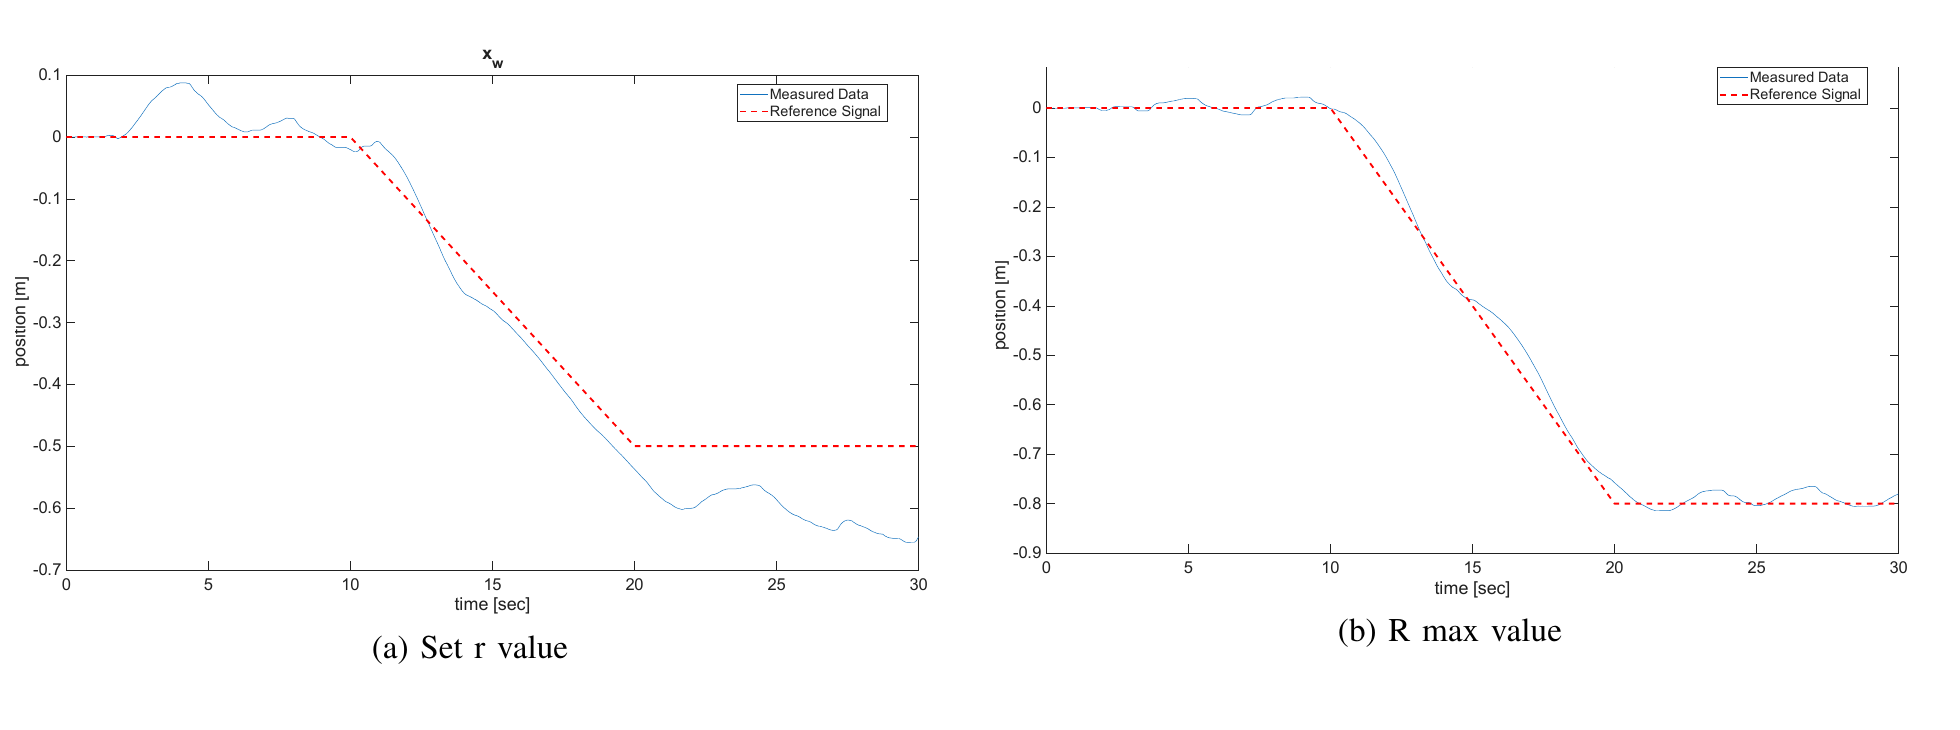
\includegraphics[width=0.92\linewidth]{../fig/findemo_combined.png}
\caption{Final-demonstration ramp-tracking test: measured $x_w$ (blue, ``Measured Data'') vs.\ commanded ramp reference $r$ (red dashed, ``Reference Signal''). (a) Standard test, ramp slope 0.05~m/s. (b) $r_{\max}$ test, ramp slope 0.08~m/s. Both track closely with 2--5~cm residual oscillation; the robot did not fall in either test.}
\label{fig:findemo}
\end{figure}

\section{Discussion}\label{sec:discussion}
\textbf{PID vs.\ state feedback.} PID only regulates $\theta_b$, leaving $x_w$ marginally stable, so drift is never corrected. Pole placement and LQR regulate both states, consistent with the PID robot falling after $\approx$20~s while the LQR-with-observer robot balanced for the full run.

\textbf{Pole placement vs.\ LQR.} Both stabilise the model; LQR was preferred mainly because weight tuning avoids guessing pole locations, and gave a smaller angle/voltage transient at the cost of the slow real pole ($-0.259$) governing $x_w$ recovery.

\textbf{Simulation vs.\ hardware.} The clearest mismatch is that the observer-inclusive simulation predicted instability below 47.6~Hz, yet the robot balanced down to $\approx$4.5~Hz. Possible causes (Section~\ref{sec:discrete}) include model conservatism, a controller/observer mismatch versus the robot, sensor filtering, or a short test window; the data do not distinguish between them.

\textbf{Actuator saturation.} Ordinary balancing used only a fraction of the $\pm9$~V rail ($\approx$5~V peak-to-peak). Under the sinusoidal reference, $v_m$ instead reached its plotted axis limits (Fig.~\ref{fig:ref3}), coinciding with the large $\theta_b$ excursions and loss of tracking.

\textbf{Observers.} The full-order observer had lower reported $\theta_b$ error than the reduced-order observer (one fewer state) in simulation; the available record does not identify which was used for the best physical run, so no hardware ranking is claimed.

\begin{table*}[t]
\centering
\caption{Summary comparison of the four control strategies. $x_w$-reg.: whether wheel position is actively regulated.}
\label{tab:compare}
\normalsize
\setlength{\tabcolsep}{6pt}
\resizebox{\textwidth}{!}{%
\begin{tabular}{@{}lllllll@{}}
\toprule
\textbf{Method} & \textbf{Gain} & \textbf{Domain} & \textbf{$x_w$-reg.} & \textbf{Test} & \textbf{Result} & \textbf{Main limitation}\\
\midrule
PID & $(K_d,K_p,K_i){=}(-0.12,-61.25,-340.23)$ & Cont.\ & No & Physical & Balanced $\approx$20/30~s, then fell & $x_w$ marginally stable\\
Pole placement & $K_{\text{pp}}{=}[-20308,-3619,-7268,-832]$ & Cont.\ & Yes & Sim.\ & Settles $\approx$1.5~s & Large transient effort\\
LQR (continuous) & $K_{\text{lqr}}{=}[-5.48,-44.33,-66.86,-10.89]$ & Cont.\ & Yes & Sim.\ & Dominant pole $-0.259$ & Slow $x_w$ recovery\\
LQR + Luenberger obs.\ & $K_d{=}[-16.14,-26.51,-87.15,-6.23]$ & Discrete, 200~Hz & Yes & Physical & Balanced full 30~s run & Fails under fast sinusoidal $r$\\
\bottomrule
\end{tabular}}
\end{table*}

\section{Conclusions}\label{sec:conclusion}
PID control kept the robot balanced for approximately 20~s of a 30~s test but did not regulate wheel position, so drift accumulated until the robot fell. The complete linearised system satisfies $\mathrm{rank}(\mathcal{C})=4$, but the angle-only model satisfies only $\mathrm{rank}(\mathcal{O})=3$ because $x_w$ is absent from the angle dynamics; measuring both $x_w$ and $\theta_b$ restores observability and enables full-order and reduced-order Luenberger state estimation. LQR combined with observer-based estimation gave the best recorded physical performance, remaining balanced for the full 30~s documented run with motor voltage well below saturation. The exact observer configuration used in the best 200~Hz physical run was not preserved in the written experimental record. Sampling-frequency results differed markedly between simulation and hardware -- a 47.6~Hz observer-inclusive simulated limit versus an approximately 4.5~Hz physical limit -- and the available data do not identify a single cause. The 200~Hz operating frequency was selected as a validated point that produced low measured tracking norms, not as a proven global optimum. The reference compensator tracked ramp references up to $r_{\max}=0.08$~m/s with small residual oscillation, but an aggressive sinusoidal reference drove the motor voltage to, or beyond, its rated limit and the robot lost tracking. Future work should log the controller and observer configuration used in every physical trial, match simulation and hardware test conditions more closely, incorporate actuator-saturation and sensor-noise models into the design, and repeat the sampling-frequency sweep with multiple trials per rate to separate genuine trends from run-to-run variability.

\section*{Acknowledgment}
The authors thank Khalid Atta and Johan Lindqvist for the laboratory framework and guidance throughout the course.

\footnotesize
\begin{thebibliography}{4}
\bibitem{luenberger} D.~G. Luenberger, ``Observing the state of a linear system,'' \emph{IEEE Trans. Military Electronics}, vol.~8, no.~2, pp.~74--80, 1964.
\bibitem{franklin} G.~F. Franklin, J.~D. Powell, and M.~L. Workman, \emph{Digital Control of Dynamic Systems}, 3rd ed. Reading, MA: Addison-Wesley, 1998.
\bibitem{anderson} B.~D.~O. Anderson and J.~B. Moore, \emph{Optimal Control: Linear Quadratic Methods}. Englewood Cliffs, NJ: Prentice Hall, 1990.
\bibitem{ogata} K.~Ogata, \emph{Modern Control Engineering}, 5th ed. Upper Saddle River, NJ: Prentice Hall, 2010.
\end{thebibliography}

\end{document}
